% This is samplepaper.tex, a sample chapter demonstrating the
% LLNCS macro package for Springer Computer Science proceedings;
% Version 2.20 of 2017/10/04
%
\documentclass[runningheads]{llncs}
%
\usepackage{graphicx}
\usepackage{hyperref}
\usepackage{color}
% Used for displaying a sample figure. If possible, figure files should
% be included in EPS format.
%
% If you use the hyperref package, please uncomment the following line
% to display URLs in blue roman font according to Springer's eBook style:
\renewcommand\UrlFont{\color{blue}\rmfamily}

\begin{document}
%
\title{A brave new algorithm \thanks{Supported by organization x.}}
%
%\titlerunning{Abbreviated paper title}
% If the paper title is too long for the running head, you can set
% an abbreviated paper title here
%
\author{First Author\inst{1}\orcidID{0000-1111-2222-3333} \and
Second Author\inst{2,3}\orcidID{1111-2222-3333-4444} \and
Third Author\inst{3}\orcidID{2222--3333-4444-5555}}
%
\authorrunning{F. Author et al.}
% First names are abbreviated in the running head.
% If there are more than two authors, 'et al.' is used.
%
\institute{Princeton University, Princeton NJ 08544, USA \and
Springer Heidelberg, Tiergartenstr. 17, 69121 Heidelberg, Germany
\email{lncs@springer.com}\\
\url{http://www.springer.com/gp/computer-science/lncs} \and
ABC Institute, Rupert-Karls-University Heidelberg, Heidelberg, Germany\\
\email{\{abc,lncs\}@uni-heidelberg.de}}
%
\maketitle              % typeset the header of the contribution
%
\begin{abstract}

At the beginning of this year one of the authors read `A brave new world` by Aldous Huxley. 
The Nobel describes a dystopia, which anticipates the development of breeding technology, 
and how this technology creates the perfect human race. Taking into account that when 
talking about genetic algorithms our goal is to achieve the optimum solution of a problem, 
and this book kind of describes the process for making the “perfect human”,  we will try to work on this
parallelism in this paper. The goal is to develop a Genetic algorithm based
on the fecundation process of the book and compare it to other algorithms to see how it behaves.
Investigating how the division in castes affects the diversity in the poblation.

\keywords{Evolutionary algorithm  \and Metaheuristics \and Another keyword.}
\end{abstract}
%
%
%

% \section{First Section}
\subsection{A Subsection Sample}
Please note that the first paragraph of a section or subsection is
not indented. The first paragraph that follows a table, figure,
equation etc. does not need an indent, either.

Subsequent paragraphs, however, are indented.

\subsubsection{Sample Heading (Third Level)} Only two levels of
headings should be numbered. Lower level headings remain unnumbered;
they are formatted as run-in headings.

\paragraph{Sample Heading (Fourth Level)}
The contribution should contain no more than four levels of
headings. Table~\ref{tab1} gives a summary of all heading levels.

\begin{table}
\caption{Table captions should be placed above the
tables.}\label{tab1}
\begin{tabular}{|l|l|l|}
\hline
Heading level &  Example & Font size and style\\
\hline
Title (centered) &  {\Large\bfseries Lecture Notes} & 14 point, bold\\
1st-level heading &  {\large\bfseries 1 Introduction} & 12 point, bold\\
2nd-level heading & {\bfseries 2.1 Printing Area} & 10 point, bold\\
3rd-level heading & {\bfseries Run-in Heading in Bold.} Text follows & 10 point, bold\\
4th-level heading & {\itshape Lowest Level Heading.} Text follows & 10 point, italic\\
\hline
\end{tabular}
\end{table}


\noindent Displayed equations are centered and set on a separate
line.
\begin{equation}
x + y = z
\end{equation}
Please try to avoid rasterized images for line-art diagrams and
schemas. Whenever possible, use vector graphics instead (see
Fig.~\ref{fig1}).

\begin{figure}
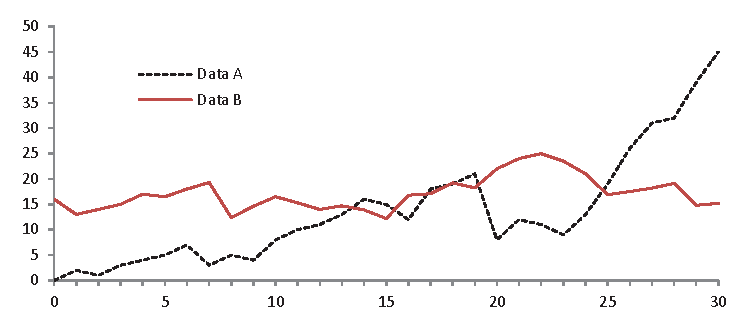
\includegraphics[width=\textwidth]{fig1.eps}
\caption{A figure caption is always placed below the illustration.
Please note that short captions are centered, while long ones are
justified by the macro package automatically.} \label{fig1}
\end{figure}

\begin{theorem}
This is a sample theorem. The run-in heading is set in bold, while
the following text appears in italics. Definitions, lemmas,
propositions, and corollaries are styled the same way.
\end{theorem}
%
% the environments 'definition', 'lemma', 'proposition', 'corollary',
% 'remark', and 'example' are defined in the LLNCS documentclass as well.
%
\begin{proof}
Proofs, examples, and remarks have the initial word in italics,
while the following text appears in normal font.
\end{proof}
For citations of references, we prefer the use of square brackets
and consecutive numbers. Citations using labels or the author/year
convention are also acceptable. The following bibliography provides
a sample reference list with entries for journal
articles~\cite{ref_article1}, an LNCS chapter~\cite{ref_lncs1}, a
book~\cite{ref_book1}, proceedings without editors~\cite{ref_proc1},
and a homepage~\cite{ref_url1}. Multiple citations are grouped
\cite{ref_article1,ref_lncs1,ref_book1},
\cite{ref_article1,ref_book1,ref_proc1,ref_url1}.
\section{Introduction}

% Introduce the problem: diversity in metaheuristics/global optimization problems
Population-based algorithms \cite{prugel2010benefits} are global optimization, stochastic
methods that use different techniques for exploring the search space
in such a way that it makes finding the solution feasible in a
reasonable amount of time. As such, they must strike a balance between
feasibility (exploitation of the features found in the current
population of solutions to optimize fitness) and off-line performance
(exploration of parts of the search space that might hold the key to
those solutions) \cite{xu2014exploration}. And in this balance,
diversity is one of the keys \cite{alba2005exploration}. This drives
the search for new algorithms that explicitly try to keep this balance
in a {\em comfort zone}.

In this search, inspiration may arrive from unexpected places.
At the beginning of the year one of the authors read the famous book
by Aldous Huxley: A brave new world \cite{huxley2007brave}. The novel
is a distopy that describes the development in reproductive
technology, psychological manipulation (including virtual-reality
plays called {\em feelies} \cite{lecakes2021matrix}) and classical
conditioning \cite{bernheim2002addiction}. It introduced interesting
ideas in several areas, but in this paper we are going to focus in how
they optimize the population.

In order to maximize efficiency and decrease unhappiness, the book
describes how the population is divided in \textit{castes}, assigned
since birth, where everyone knows and accepts their place. That way,
they achieve an ``optimum world``, whose optimization is based on
these reproduction restrictions and in the overall balance the division in
castes creates, not in an individual. This tension between the
individual happiness or realization and the overall harmony or optimal
state is, precisely, the main plot driver, becoming a literary
harbinger of the comparison between individual and population-based
optimization algorithms, although of course the intention of the
author was to compare collectivist and individualist culture
\cite{mathews2012happiness}.

When we talk about evolutionary algorithms the target is reaching the
optimum solution for a problem, and this books perfectly describes
the process through which they have reached the perfect human
race. Therefore we want to develop an algorithm based on the book's
fecundation proceses and compare its behaviour with other
algorithms. Our main assumption during the design of this process is
that the division in castes affects the
poblation's diversity; we can draw a parallel between the
collectivism/individualism tensions inherent in the novel and the
exploration/exploitation balance in population based global
algorithms, and thus try and apply their solutions to our
problems. The main conclusion we draw from the book is that what makes
collective society happy might make some individuals extremely
isolated and sad; but if we apply this to our optimization realm we
can see that what Aldous Huxley might be unwittingly proposing is the
rough layout of an optimization algorithm, where individuals with 
different fitnesses undergo different
differentiation/evolution/reproduction processes. We will take it from
here to design an optimization algorithm, which of course we call Brave
New Algorithm.

When designing an algorithm from scratch, we must also make technical
choices on how this implementation is going to take place, as well as
how the whole process of going from design (our {\em user stories}) to
final implementation (product) can be performed according to best
practices in software engineering. Implementation matters
\cite{merelo2011implementation}, and an agile development process can
help us get the final result in the most efficient way, guaranteeing
the quality of any software product \cite{DBLP:journals/corr/abs-2104-12545}.

The rest of the paper is organized as follows: next, the state of the
art in this area is examined. The algorithm (and its implementation)
are described in \ref{sec:algorithm}. The first experiments performed
with this implementation of the algorithm are shown in
\ref{sec:experiments}. Finally, we will discuss the results and
present our conclusions in Section \ref{sec:conc}.
\section{State of the art}


% What's the point of new metaheuristics.
One of the {\em koans} written by Goldberg in ``Zen and the art of the
evolutionary algorithm'' states that we should Nature be our guide. This has
profitably led to many different population-based metaheuristics that are
inspired by the behavior of different species \cite{nedjah2020inspiration}, going as far as the behavior of
pigeons in a park \cite{blanco2019urban}. The exhaustion of the pool of
species with collective behavior to mimick has led further away, for instance to
zombies \cite{nguyen2012zombie}, which eventually has led to backlash
\cite{metaphor_exposed} claiming how metaphors obscure understanding of new
algorithms, and do not advance the field of optimization. In fact, evolutionary
algorithms are not the best way to reflect social processes
\cite{chattoe1998just}, but in this case the intent of Aldous Huxley was exactly
the opposite: how an industrial, at scale, version of biological evolution
applied to the whole human race (except for the what they called ``savages'')
could determine social processes.

This does not imply, however, that metaphors are necessarily
unhelpful. The potential of a book such as the one we deal with here to inspire
optimization has, however, not been realized, although it has been
mentioned at least one in relation with an evolutionary algorithm:
\cite{wollam1999reverse} mentioned one of the ``methods'' of the book,
``screening out savages'', as a way of, apparently, giving 0 fitness
to missiles that didn't meet the constraints of a ``commanded flight
profile''.

% How does diversity influence search and what type of problems is
% going to profit from it
Curiously enough, another oblique reference to Brave New World via the
sentence
\begin{quote}
  Consider the horse. They considered it.
  \end{quote}
in \cite{DBLP:journals/corr/abs-2107-00314} brings us to the main
theme in this paper. By ``considering the horse'', the author of the
novel refers to how exploration, the enhancement of diversity, is able
to find new solutions to problems.

% What other efforts have been made in this area
\section{Algorithm's Nature}

As it was mentioned before, the algorithm is based in the optimization's process of the human race described on the book, thus we
are talking about an algorithm based in the evolution of a population, it will follow the structure of evolutionary algorithms
specifically a \textit{genetic algorithm}. The book describes how they achieved the perfect human race working with an assembly 
line with different phases. This will be reflected with a \textit{generational evolutionary algorithm} with selection, 
crossover, mutation and replacement operators.

The process begins in the \textbf{\textit{Fecundation Room}}, here the eggs are created and fertilized. Once the fertilization
is finished all the eggs got to the \textbf{\textit{Hatchery}} where the caste to which each individual will belong is decided. 
Huxley describes how the higher castes (\textit{Alpha} and \textit{Beta}) are suministred a higher amount of nutrients and hormones during the 
incubation. While the lower castes (\textit{Gamma}, \textit{Delta}, and \textit{Epsilon}) are deprived of these elements, needed for the development.
To imitate this ``lack of nutrients``, in the algorithm developed we will deprive the lower castes of the operators, they will only mutate. 
With all that has been mentioned, the castes will be developed in the following way :

\begin{itemize}
    \item \textbf{Alphas}: in the books they are the most intelligents, the elite belongs to this group. They have responsibilities, they are
    ones that take decisions. In our implementation they will be reproduced with other individuals of the caste and they will evolve with
    all the operators.
    \item \textbf{Betas}: in the book they are less intelligents that the before mentioned and their main role is working in administrative tasks.
    In the implementation, the crossover will only be with individuals from the Alpha caste,
    \item \textbf{Gammas}: in the book they are subordinates, whose tasks require hability. In the implementation they will only mutate, but using local
    search
    \item \textbf{Deltas} and \textbf{Epsilons}: in the book both these castes are employees of the other castes and do repetitive works. In the 
    implementation they will only have mutation by fixed segment. 
\end{itemize}

With this structure in min the metaheuristic will be divided in the following phases :

\begin{itemize}
    \item \textbf{Fecundation room}: the individuals are created in a randomized way.
    \item \textbf{Hatchery room}: in this phase we will divide the population in castes. We will do this following the fitness value
    of the individual as the criteria. Furthermore, each caste will have a different population percentage. Because in the book they
    mention that lower castes are produced with the \textit{Bokanovsky's process}, where an ambryo its divided into 96 identical twins.
    In the algorithm this will be reflected in the population size, that will descende when the caste is higher.
    \item \textbf{Caste evolution}: each caste will follow a different process, as it was mentioned before
\end{itemize}

We are not talking about static castes, they are generated at the beginning of each generation. Let's imagine that we have a poplation size of ten, 
each individual with a fitness value. In the fist iteration the population will be divided following that value. After that, each individual will 
follow the evolution process corresponding to the caste. At the end of each generation all the chromosomes will be mixed, regardless of the caste. The
next generation will start dividing this chromosomes in castes again. 

\section{Experimental results}
\label{sec:experiments}

In this section we will run some experiments in order to see how the algorithm
behaves regarding diversity.  First we will establish which metric will be
used to measure it. Then we will analyse the brave new algorithm, and compare
it to a basic genetic algorithm with no castes division.

\subsection{Diversity analysis}

Mantaining the \emph{diversity} is crucial for avoiding the early convergence to local optima. Rosca \cite{Rosca} concluded that 
the poblations seem to get stuck in a local optima when the entropy didn't change or decreased drably in sequential generations.
In genetic programming when we talk about diversity we refer to the structural differences such as the amount of different
genotypes in the population or the singularity of the fitness values \cite{genetic}. In this section we will analyze the diversity of our
algorithm to study how division in castes affects.

There are different ways of calculating the diversity: genotypic diversity, fenotypic diversity, entropy, pseudo-isomorphism, edit distance, etc.
Among which we chose \textit{entropy}, that describes the distribution of the poblation around the different fitness values, and the \textit{edit distance},
in which each individual it's evaluated against the best individual found so far. These metrics has been chosen since according to Burke \cite{diversity} entropy
and edit distance show a great correlation with the increment and decrement of the fitness value.

\subsection{Diversity in Brave new algorithm}

For these experiments we will use the configuration shown in Table
\ref{tab:config_file_10}. The fitness functions evaluated will be the Rastrigin
function from the \emph{Black-box optimization benchmarking} \cite{BBOB}. This
is a multimodal function, that allows to check the behavior of the algorithm in
this kind of problems and is especially appropriate to check if diversity is
maintained; a loss of diversity will make the algorithm perform poorly on this
function.

\begin{table}[]
    \caption{Configuration parameters for the diversity exploration}
    \label{tab:config_file_10}
    \centering
    \begin{tabular}{|l|l|}
        \hline
        Configuration parameters &  Value \\
        \hline
        Chromosome size                   & 20      \\ \hline
        Population size                   & 100     \\ \hline
        Maximum generations               & 15      \\ \hline
        Alpha population percentage       & 10      \\ \hline
        Beta population percentage        & 20      \\ \hline
        Gamma population percentage       & 20      \\ \hline
        Delta population percentage       & 20      \\ \hline
        Epsilon population percentage     & 30      \\ \hline
        Mutation rate for all castes      & 10      \\ \hline
\end{tabular}
\end{table}

In Figure \ref{fig:best_restrigin_diversity} the data has been taken from the Rastrigin execution that returned the best
fitness value. In the graphic on top we have the fitness value that resulted from each generation. As we can see the 
edit distance metric is closely related to the top graphic. The smallest edit distance is in the last generation, so we
can conclude that the lower the edit distance the higher possibility of the algorithm to get stuck in a local optima. 

\begin{figure}[]
	\centering	
	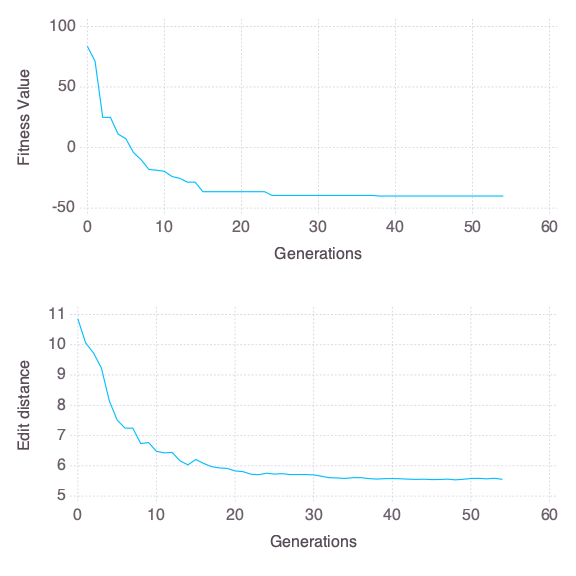
\includegraphics[scale=0.5]{./figures/config_file_10_Rastrigin_diversity.png}
	\caption{ Diversity in the execution with the best fitness value for the Rastrigin function }
    \label{fig:best_restrigin_diversity}
\end{figure}

Now let's compare the entropy for the best and worst execution of the Rastrigin function to see if the entropy has 
anything to do with the algorithm outcome. As we know, algorithms seem to get stuck in local optima when
entropy doesn't change or decrease drably in sequential generations. In Figure \ref{fig:rastrigin_diversity_comparation} we can see
this case in the execution with the worst fitness value. The entropy decreases more than 2 points from generation 0 to generation 30.
Whilst in the case of the best execution the entropy slope is less strong. Also in the execution with the best fitness we can see how
when the entropy stays with similar values for multiple generations is when it gets stucked in local optima.

\begin{figure}[]
	\centering	
	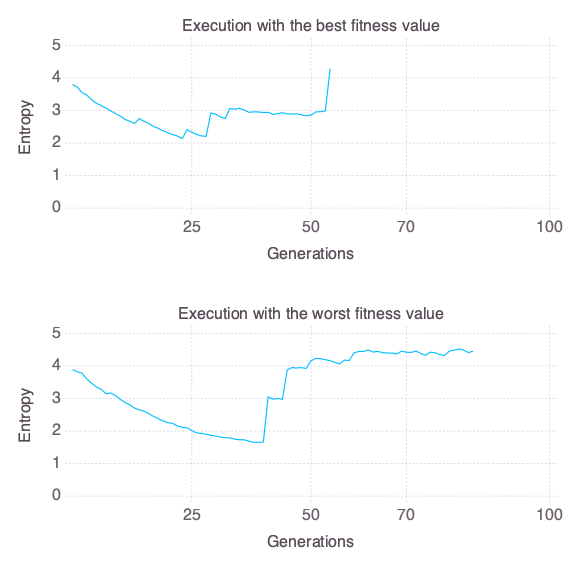
\includegraphics[scale=0.5]{./figures/config_file_10_Rastrigin_diversity_comparation.png}
	\caption{ Comparation of the diversity between the execution with the best and the worst fitness value for the Rastrigin function }
    \label{fig:rastrigin_diversity_comparation}
\end{figure}

With this information we can now compare the diversity of our algorithm with the behaviour of a genetic algorithm without
castes division.

\subsection{Diversity on a basic genetic algoritm}

We will now compare the diversity of the Brave new algorithm with a ``basic`` genetic algorith, meaning an algorithm without castes division, in order
to check how the division affects the diversity.

In Table \ref{tab:diversity_comparation} we can see the results comparation for both algorithms. Having a higher value on
the entropy standard deviation means that the values are spread out over a wider range, this is the case for the Brave
new algorithm. Also, it has a better median of the fitness value. In Figure \ref{fig:rastrigin_diversity_comparation} we can see
how the entropy in the basic algorithm looks like more variant, but the values are only between 5 and 5.5.

For this section we can conclude that because the Brave new algorithm has a higher standard deviation on the entropy the 
diversity is mainted throught more generations that for the basic genetic algorithm, resulting in better median for the fitness value.

\begin{table}[]
    \centering
    \caption{Entropy results for Brave New Algorithm (BNA) and a genetic algorith without castes division (GA)}
    \begin{tabular}{|c|c|c|c|c|}
    \hline
    \textbf{Algorithm} & \textbf{\begin{tabular}[c]{@{}c@{}}entropy\\ median\end{tabular}} & \textbf{\begin{tabular}[c]{@{}c@{}}f. value\\ median\end{tabular}} & \textbf{entropy $\sigma$} & \textbf{f. value $\sigma$} \\ \hline
    BNA                & 2.9                                                               & -39.56                                                             & 0.41             & 26.12             \\ \hline
    GA                 & 5.27                                                              & 528.21                                                             & 0.01             & 224.09            \\ \hline
    \end{tabular}
    \label{tab:diversity_comparation}
\end{table}

\begin{figure}[]
	\centering	
	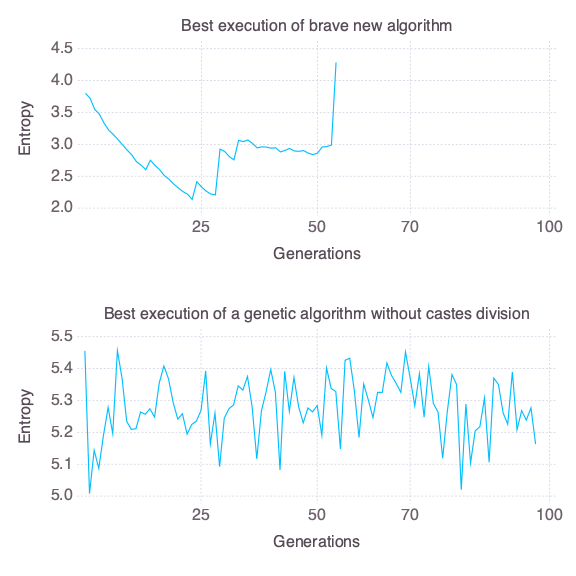
\includegraphics[scale=0.5]{./figures/Rastrigin_diversity_algs_comparation.png}
	\caption{ Comparation of the diversity between the best executions of the Brave New Algorithm and a genetic algorith without castes division }
    \label{fig:diversity_comparation}
\end{figure}




%
% ---- Bibliography ----
%
% BibTeX users should specify bibliography style 'splncs04'.
% References will then be sorted and formatted in the correct style.
%
% \bibliographystyle{splncs04}
% \bibliography{mybibliography}
%
\bibliographystyle{splncs04}
\bibliography{brave-new-algorithm}

\end{document}
